
\section{Engine Extensions}


\subsection{Tile Extension}


\subsubsection*{Vision}

As the basic rules for which tiles can be seen from where have been
explained in the System Features section, we will now turn our attention
to how corners are connected with each other. 

Recall that a corner $c_{1}$ on a tile $t_{1}$ connects to a corner
$c_{2}$ of another tile $t_{2}$ if a straight line can be traced
from $c_{1}$ to $c_{2}$ without intersecting with a tile that is
blocking the line. In the tile extension, a tile is blocking the line
if it contains an entity that is movement blocking with respect to
the entity looking from $t_{1}$. Additionally, the tile $t_{2}$
is visible from $t_{1}$ if at least one corner of $t_{1}$ connects
to at least three corners of $t_{2}$. If $t_{2}$ is vision blocking,
only two corners of $t_{2}$ need be connected to. In its most simple
form, the algorithm iterates over all the tiles in the agent's visible
range, and returns a collection containing just those satisfying the
above condition. 

The interesting part of the algorithm is this: how do we find all
the tiles a line from one corner to another passes through? \texttt{\emph{{[}Figure{]}}}
To accomplish this, we find the slope of the line as $\left|\frac{v_{x}}{v_{y}}\right|$,
where $v$ is the vector describing the line. If either $v_{x}$ or
$v_{y}$ is zero, the line only passes between tiles, and it is handled
as a special case.

\texttt{\emph{{[}Explain that it is similar to that other algorithm
(name?){]}}}


\subsection{EIS Extension}

EIS support to the engine to the engine is provided with a special
\texttt{AgentController/AgentManager }class, along with a specially
designed java EIS environment jar file. This section will go through
how the implementation works and how we connect to the EIS environment.

The EIS environment in java and the agent controller on the engine
is connected through a TCP connection. They commicate with each other
with XML as a markup language for the data they transmit. 

Fig. \ref{fig:DeploymentEISandAgentController} shows the setup between
EIS and the agent controller.

\begin{figure}
\begin{centering}
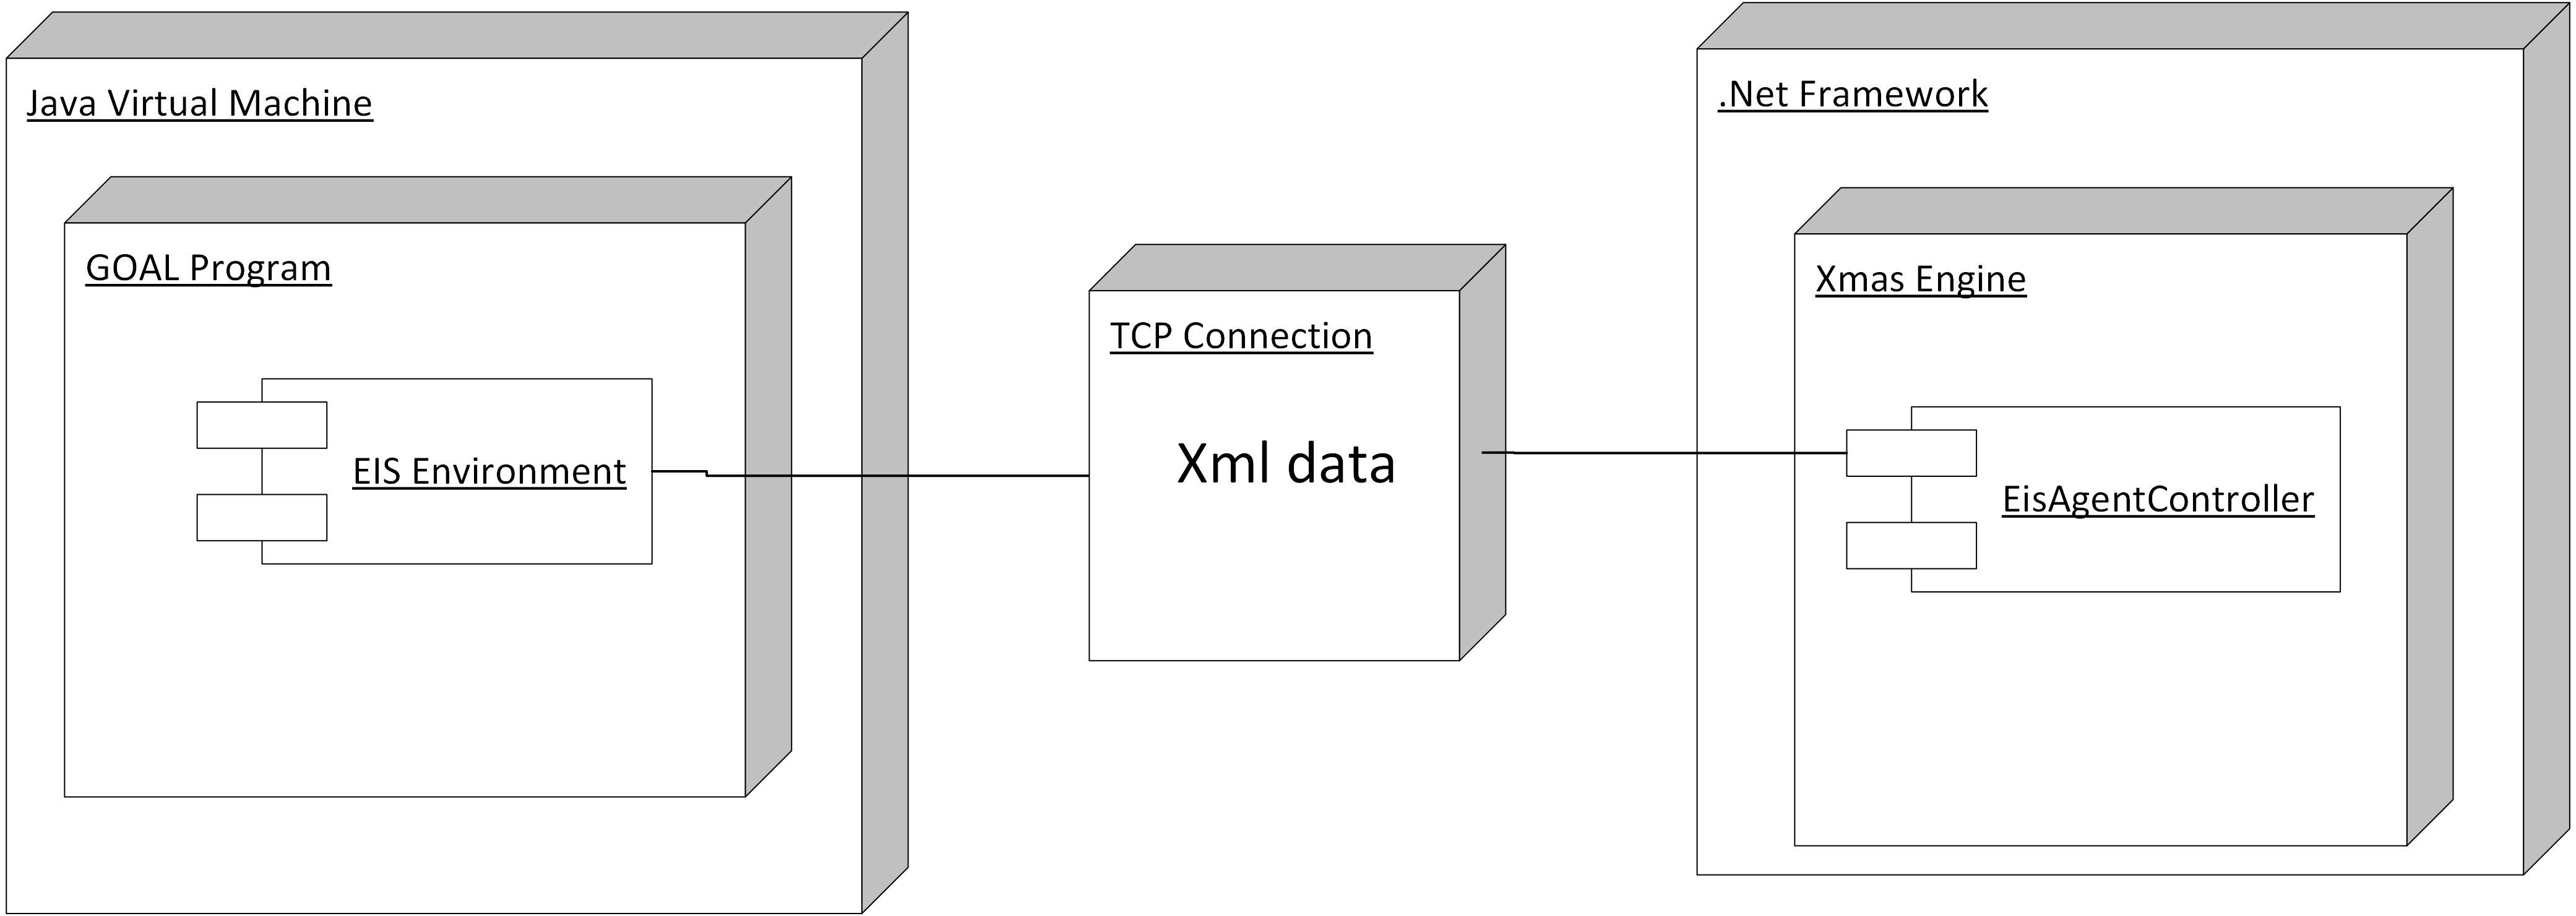
\includegraphics[width=1\textwidth]{DeploymentEISandAgentController}
\par\end{centering}

\caption{An illustration of the connection between the EIS environment and
the agent controller.\label{fig:DeploymentEISandAgentController}}


\end{figure}


Although the EIS environment and the agent controller sends all data
in form of XML data there is one difference and that is all XML nodes
are packaged into packages of a certain size and the size is sent
before the xml data, as can be seen in fig. \ref{fig:DataPackaging}.

\begin{figure}
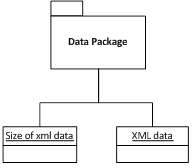
\includegraphics[scale=0.8]{XMLDataPackageFigure}

\caption{Image of the data sent between the EIS environment and the agent controller.\label{fig:DataPackaging}}


\end{figure}


This was done to ensure that the agent controller at all times knew
how much data was to be transmitted, thus giving it the right to deny
packages if they were over a certain size. In our current implementation
however no package size is denied. 


\subsubsection*{Engine Side of EIS Support}

In the project: \texttt{XmasEngineExtensions }we provide two classes:
\begin{description}
\item [{\texttt{EISAgentController:}}] this class is responsible for converting
xml data from the EIS environment into actions that can be queued
to the agent it controls. And also for converting percepts the agent
it controls receives into XML data that can be sent to the EIS environment.
\item [{\texttt{EISAgentServer}}] creates a TCP server all EIS environments
that wishes to connect to it must make a TCP client call, once a connection
is established then the agent server will construct an \texttt{EISAgentController
}object, that object will take over all further duties of comuncation.
\end{description}

\subsubsection*{How the EISAgentServer works}

The server manages the agent controllers and it also manages the connection
creation between an EIS environment and an \texttt{EisAgentController}.

On Fig. \ref{fig:EISServerSequenceDiagram} is shown how an EIS environment
connects to an agent server and how the agent server handles the connection.
The connection works by the EIS environment making a TCP connection
request the agent server then responds by constructing the agent controller(
and give it, its own thread). Once the agent controller is constructed
the agent server is no longer responsible for handling that connection
and leaves it up to the agent controller to find out what the EIS
environment wants. This is basically to connect to a given agent whom
it knows by name, and start sending it actions.

\begin{figure}
\begin{centering}
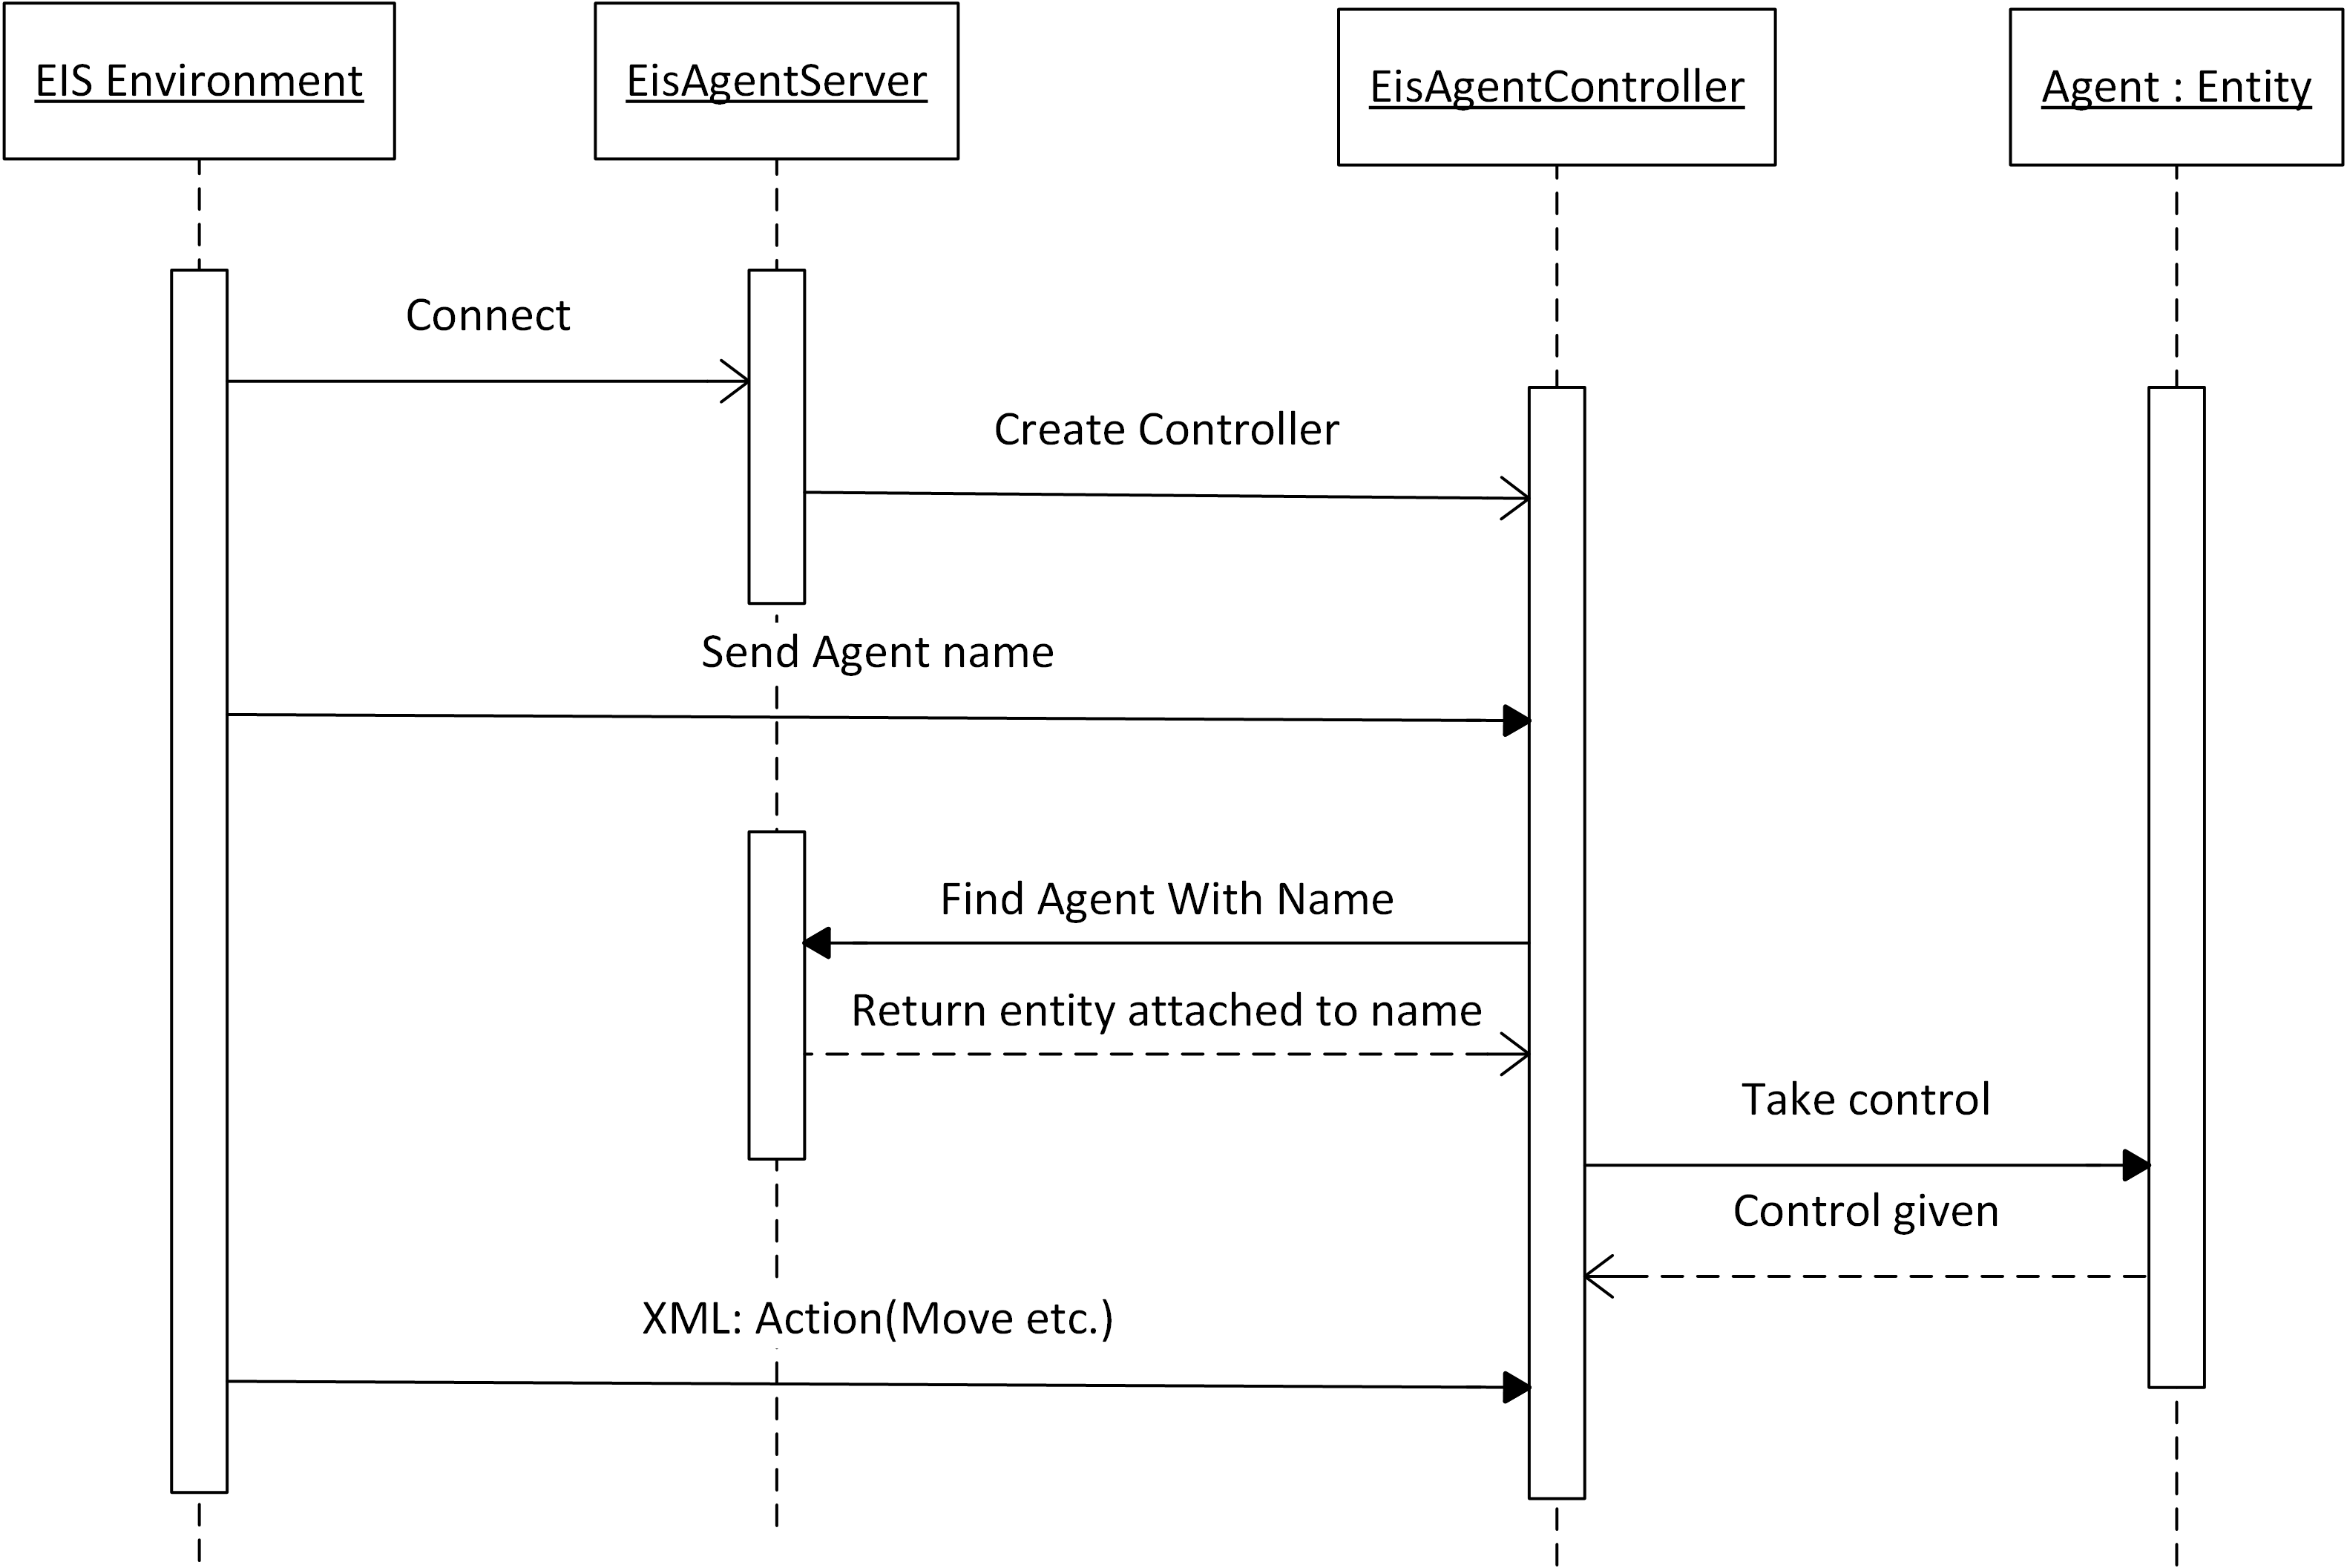
\includegraphics[width=1\textwidth]{EISServerSequenceDiagram}
\par\end{centering}

\caption{a sequence diagram of an EIS environment connecting to the engine
through an EisAgentServer.\label{fig:EISServerSequenceDiagram}}


\end{figure}



\subsubsection*{How the EisAgentController works}

The EIS agent controller job is to ensure that all demands made by
an EIS environment is fulfilled, this is done by receiving actions
in XML data form, and convert the data into Xmas Actions. These actions
are then queued onto an agent.

\begin{figure}
\begin{centering}
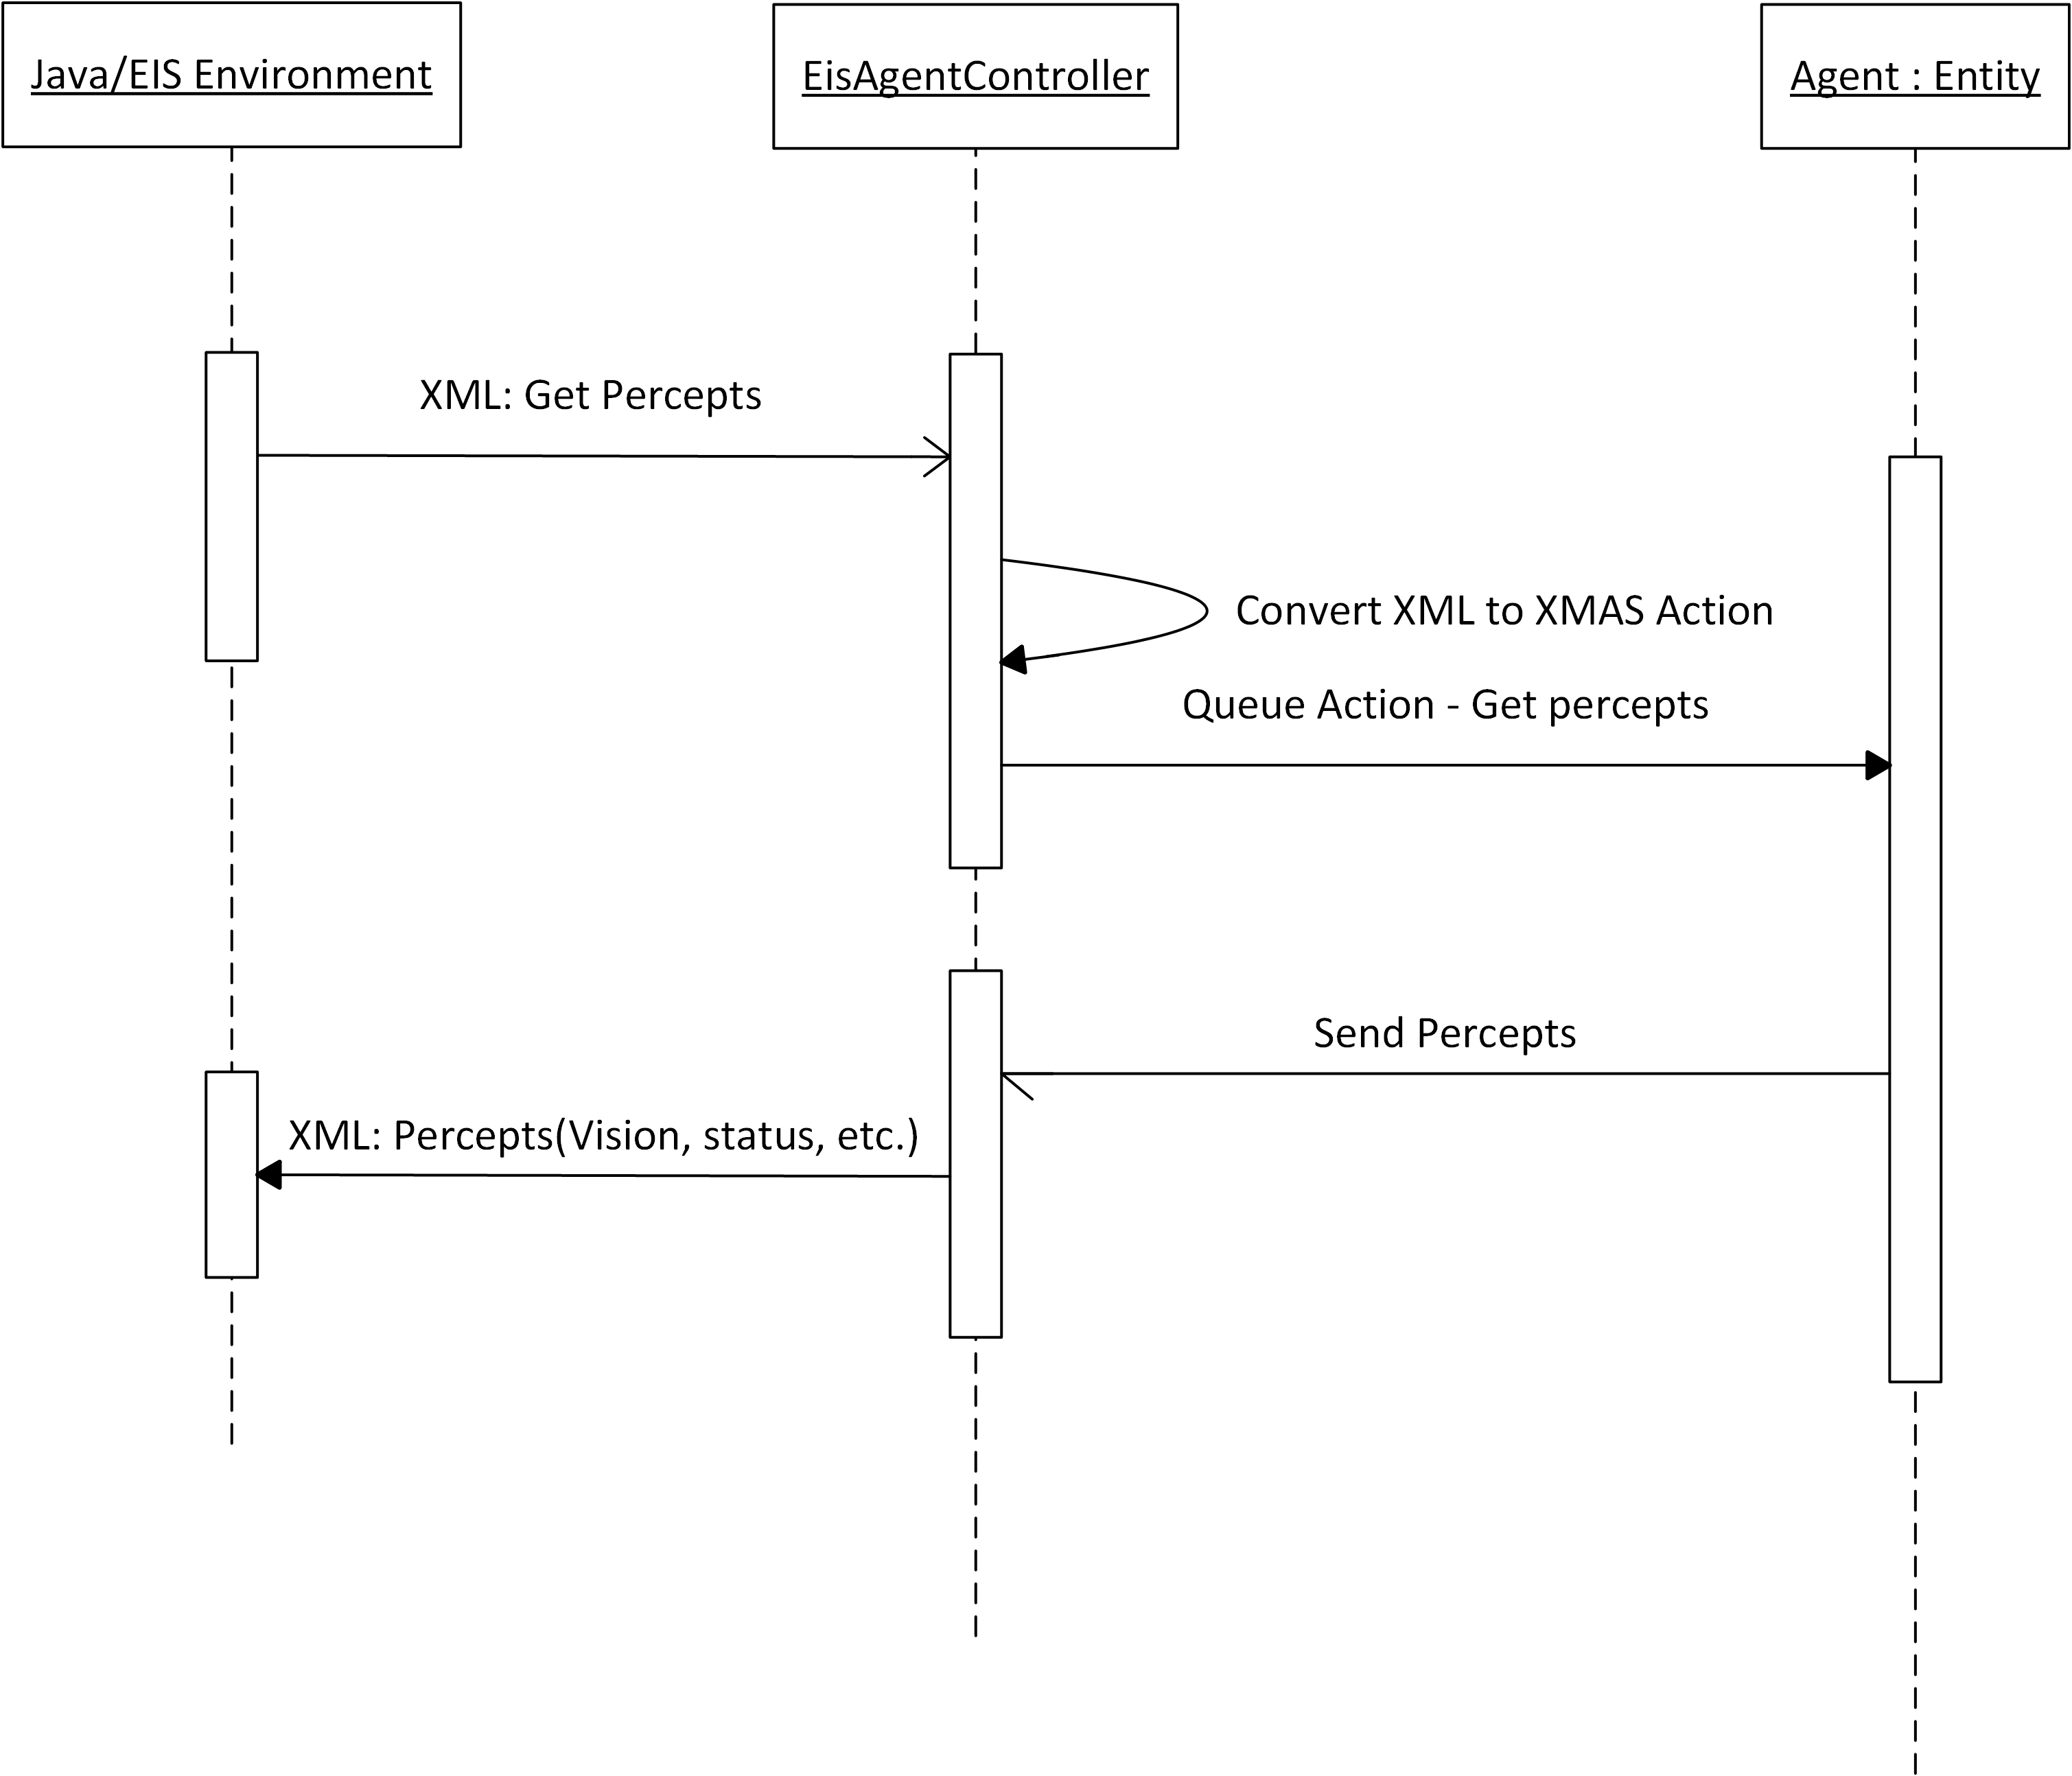
\includegraphics[width=1\textwidth]{EisAgentControllerSequenceDiagram}
\par\end{centering}

\caption{A sequence diagram showing how XML data from EIS environment are converted
into Xmas data.\label{fig:EisAgentControllerSequenceDiagram}}


\end{figure}


On fig. \ref{fig:EisAgentControllerSequenceDiagram}, is shown how
xml data received is converted by the controller and then sent to
the agent inside the engine. Percepts are only sent if they are updated
in this case the action was to get percepts however if the action
was to move an agent, then no percepts would be sent the controller.


\subsubsection*{EIS Environment}

The EIS environment is designed to setup an interface between an APL
and an environment built in java. As our engine is built In C\#, we
cannot use the EIS as it was supposed to. The way we use EIS instead
is by making it a hollow link between our engine and the APL(such
as GOAL). Thus the EIS environment implementation we make must be
able to provide communication between the APL and our engine. The
way we have done this is by making the environment convert all the
XML data it receives into the EIS data-structures for percepts. Which
is one of the classes that EIS provides, it all provides the means
to directly convert the data structures into prolog code which is
used by GOAL to understand the data.

\begin{figure}
\begin{centering}
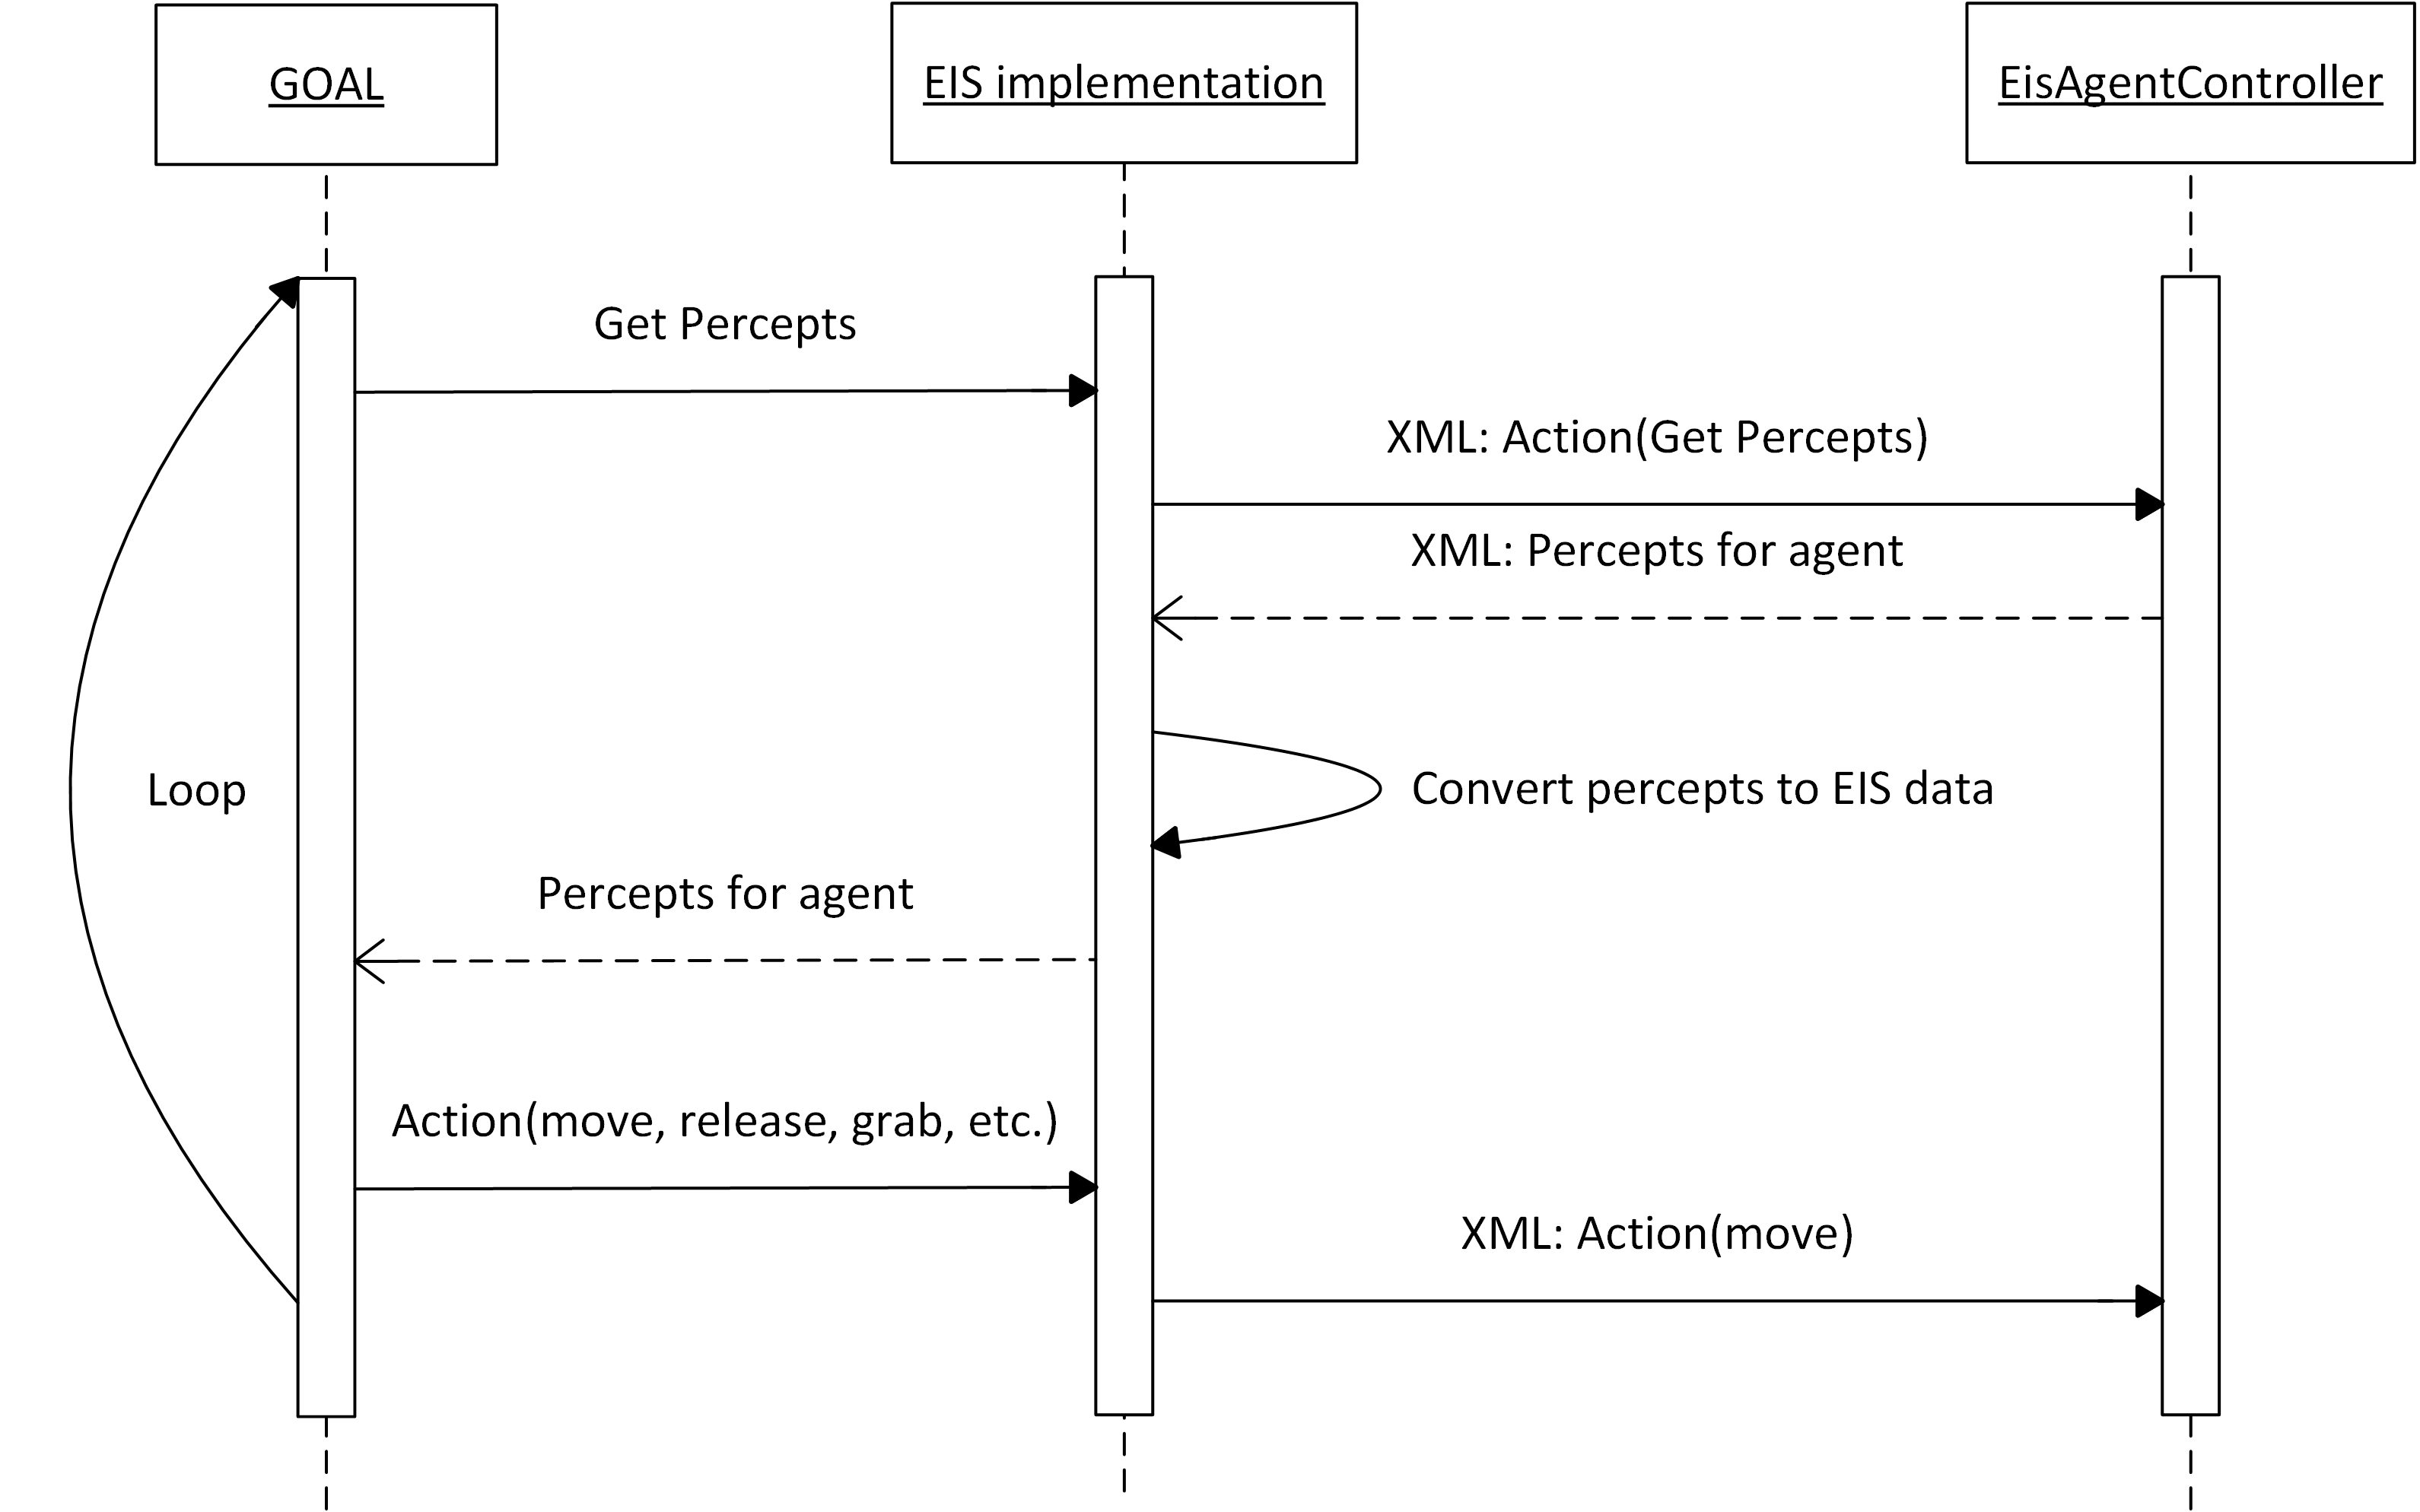
\includegraphics[width=1\textwidth]{EISEnvironmentToGoalSequenceDiagram}
\par\end{centering}

\caption{This diagram shows how the communication between goal and the EIS
environment works.\label{fig:EISEnvironmentToGoalSequenceDiagram}}


\end{figure}


An example of sequence for the EIS environment communicating with
an APL(such as GOAL) can be seen on fig. \ref{fig:EISEnvironmentToGoalSequenceDiagram}.
The basic idea is that the goal program sends commands directly to
the EIS environment we have implemented and then we ensure that those
commands are fulfilled by transmitting them over to the \texttt{EisAgentController},
through a TCP connection.


\subsection*{Considerations}

The design of interfacing with goal was originally what the engine
design was mostly focused on; as such there have been lots of different
approaches to this interfacing that we have gone through. One approach
was to connect the EIS environment using J\# which could be converted
into C\# byte code; this would be a lot faster than our current approach
since XML data wastes a lot of space by encapsulating every bit of
information. However J\# is an old language and we wanted to ensure
that we did not run into too many complications under development
as such we chose our current approach since the real time transmission
of data is not as important as the idea of it, for this project in
particular. 


\subsection*{Summary}

EIS is an interface for designing environments in java that connects
to EIS supported APLs, we use this environment to develop an environment
that is simply a TCP connection between the APL(in our case goal)
and our engine. The design provides the necessary features to the
engine, but the design could have been more optimized by using a more
compact way of sending data, since sending data as XML nodes takes
up a lot of space since XML requires all data to be encapsulated by
it.
